\documentclass[a4]{article}
\usepackage{geometry}
\geometry{verbose,tmargin=2.5cm,bmargin=2.5cm,lmargin=3cm,rmargin=3cm}
\usepackage{amsmath,amssymb,amsthm}
\usepackage{graphicx}
\graphicspath{{graphics/}}
\usepackage[utf8]{inputenc}
\usepackage{fancyvrb}
\usepackage{hyperref}
\usepackage{lscape}
\usepackage{adjustbox}
\usepackage{verbatim}
\usepackage{subcaption}
\usepackage{placeins}


\title{MultiFEBE \\ ME-TH-CO-001 [TUTORIAL] \\ Impedances of inclined pile foundations (BEM-FEM model)}

\author{\'A.G. Vega-Artiles}

\date{March 2023}

\begin{document}

\maketitle

\tableofcontents 

\section{Problem description}

In this seventh tutorial, the impedances of different floating piles are obtained. Firstly, a model with a single inclined pile will be studied and then a $2 \times 2 $ group of piles. 
 
\section{Single battered pile}

In this section, the horizontal, horizontal–rocking crossed and rocking impedances of a single battered pile will be calculated by subjecting pile heads to forced vibration in each of the oscillation modes. This process will be done for different angles between the pile axis and the vertical \cite{padron}.

Figure \ref{fig:geometry_single_battered_pile} shows the geometry of a single battered pile. Required material and geometric properties are the Young's modulus $E$, the Poisson's ratio $\nu$, the density $\rho$, the shear modulus $\mu$, the hysteretic damping $\xi$, the pile length $L$ and the pile diameter $D$. Self-weight is not considered.

The following equations will be used: 

\begin{equation}
	\begin{array}{l}
		a_0 = \omega d/c_s \medspace \mathrm{(dimensionless)} \\
		c_s = \sqrt{\mu_s/\rho_s}\medspace \mathrm{(m/s)} \\
		\mu_s = E_s/2(1+\nu_s)\medspace \mathrm{(N/m^2)} \\
		E_p/E_s= 10^3 \medspace \mathrm{(dimensionless)} \\
		\rho_p/\rho_s=0.7 \medspace \mathrm{(dimensionless)}
	\end{array}
\end{equation}

The problem is solved for $L=15$ $\mathrm{m}$, $D=1$ $\mathrm{m}$, $E_p/E_s= 10^3$, $\nu_s=0.4$, $\rho_s=1$ $\mathrm{kg/m^3}$, $\xi_p=0.01$ and  $\xi_s=0.05$.

\begin{equation}
	\begin{array}{l}
		\mu_s = 0.3571 \medspace \mathrm{N/m^2} \\
		c_s = 0.5976 \medspace \mathrm{m/s} \\
		\rho_p = 1.4286 \medspace \mathrm{kg/m^3} \medspace \Longrightarrow \rho_p (reduced) = \rho_p - \rho_s = 0.4286 \medspace \mathrm{kg/m^3}\\
		a_0 = 0.001 \medspace \Longrightarrow \omega = 0.005976 \medspace \mathrm{rad/s}\\
		a_0 = 1 \medspace \Longrightarrow \omega = 0.5976 \medspace \mathrm{rad/s}
	\end{array}
\end{equation}

\subsection{GEO file}

The Gmsh language allows to define parameters to use later in the script and comments as every other programming language. 

In this example several parameters are defined: the pile diameter (D), the pile length (L), the angle of inclination with respect to the Z axis ($\theta$), the pile mesh element size (ms\_pile), the mesh element size for the free surface near the pile (ms\_near), the mesh element size for the free surface far from the pile (ms\_far), the radius of the free surface (R\_truncation) and the coordinates of the pile head (xp, yp) regarding always the z coordinate (zp) equals 0. 

Every point in the geometry can be specified by its coordinates (x y z) and mesh element size with the function ``Point". Every straight line of the model is created with the function ``Line" and its initial and final points. Then, with the function ``Physical Line" every line is converted into a single entity or physical entity with its own name. Furthermore, the function ``Transfinite Line" explicitly defines the location of the nodes on the line by following the expression specified and the function ``Round" rounds values to the nearest integer. Every surface is created with the function ``Plane Surface" by setting its perimeter with the function ``Line Loop" and the lines used to close the surface. Moreover, with the function ``Physical Surface" every surface is converted into a single entity or physical entity with its own name.  

It is worth noting that “if an expression defines a new entity, it is enclosed between parentheses but if an expression refers to a previously defined entity, it is enclosed between braces.” \cite{gmshweb}

Finally, the mesh generation, the element order and the *.msh file saving can also be specified with the expressions ``Mesh + mesh dimension", ``SetOrder + element order" and ``Save + name.msh", respectively.

The resulting *.geo file applied to the problem is the following:

\begin{Verbatim}
// Geometry & mesh parameters
D = 1;
L = 15;
theta = 0;
ms_pile = 2.5;
ms_near = 3;
ms_far = 5;
R_truncation = 2*L;

theta = theta*Pi/180; 
xp = 0;           
yp = 0;

Point (1) = {xp,yp,0,ms_pile};
Point (2) = {-L*Sin(theta),0,-L*Cos(theta),ms_pile};
Line  (1) = {1,2};
Transfinite Line{1}=Round(L/ms_pile+1.);
Physical Line ("line-load") = {1};

Point (3) = {xp,yp,0,ms_pile};
Point (4) = {-L*Sin(theta),0,-L*Cos(theta),ms_pile};
Line  (2) = {3,4};
Transfinite Line{2}=Round(L/ms_pile+1.);
Physical Line ("pile") = {2};

Point (5) = {            0 ,            0 , 0 , ms_near };
Point (6) = { R_truncation ,            0 , 0 , ms_far };
Point (7) = {            0 , R_truncation , 0 , ms_far };
Point (8) = {-R_truncation ,            0 , 0 , ms_far };
Point (9) = {            0, -R_truncation , 0 , ms_far };

Line  (3) = {5,6};
Circle(4) = {6,5,7};
Line  (5) = {7,5};
Line Loop (6) = {3,4,5}; 
Plane Surface(1) = {6};

Line  (7) = {8,5};
Circle(8) = {7,5,8};
Line Loop (9) = {7,-5,8}; 
Plane Surface(2) = {9};

Line  (10) = {9,5};
Circle(11) = {8,5,9};
Line Loop (12) = {10,-7,11}; 
Plane Surface(3) = {12};

Circle(13) = {9,5,6};
Line Loop (14) = {-10,13,-3}; 
Plane Surface(4) = {14};

Physical Surface("free-surface") = {1,2,3,4};

// Mesh generation
Mesh 2;
SetOrder 2;
Save "single_pile.msh";
\end{Verbatim}

\begin{figure}[h]
	\centering
	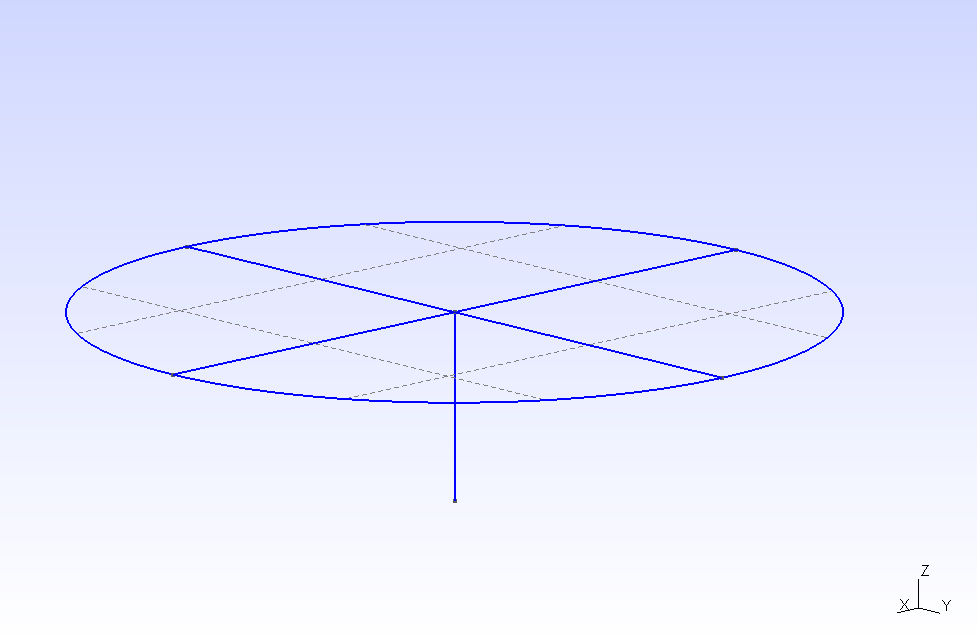
\includegraphics[scale = 0.58]{geometry.png}
	\caption{Geometry of the single battered pile resulting from the *.geo file.} 
	\label{fig:geometry_single_battered_pile}
\end{figure}

\subsection{MSH file}

The *.msh file begins with a mandatory section about information of the file (MeshFormat) and following by the other sections. Here, three sections are used: the physical group names (PhysicalName), the nodes (Nodes) and the elements (Elements).

In the section ``PhysicalName", all the physical entities of the model are defined. The first line indicates the number of physical entities. Then, one line per physical entity indicating the physical dimension, the tag and the name.  

In the section ``Nodes", all the nodes of the model are defined. The first line indicates the number of nodes. Then, one line per node indicating the node identifier and its coordinates (x y z).

In the section ``Elements", all the elements of the model are defined. The first line indicates the number of elements. Then, one line per element indicating:

\begin{itemize}
	\item Element identifier.
	\item Type of element.
	\item Number of auxiliary tags.
	\item List of tags, where the two first auxiliary tags are mandatory, and the first one corresponds to the identifier of the physical entity to which the element belongs and the second one is the identifier of the elementary model entity to which the element belongs. The rest of the tags are optional.
	\item A list of identifiers corresponding to the nodes of the element.
\end{itemize}

For example, in this case, an element with the identifiers 1 8 2 1 1 1 10 15 corresponds to:

\begin{itemize}
	\item 1: element 1.
	\item 8: type 8 (3-node second order line).
	\item 2: it has 2 auxiliary tags.
	\item 1: it belongs to the physical entity 1.
	\item 1: it belongs to the line 1.
	\item 1, 10, 15: it connects the nodes 1, 10 and 15.
\end{itemize} 

\begin{figure}[h]
	\centering
	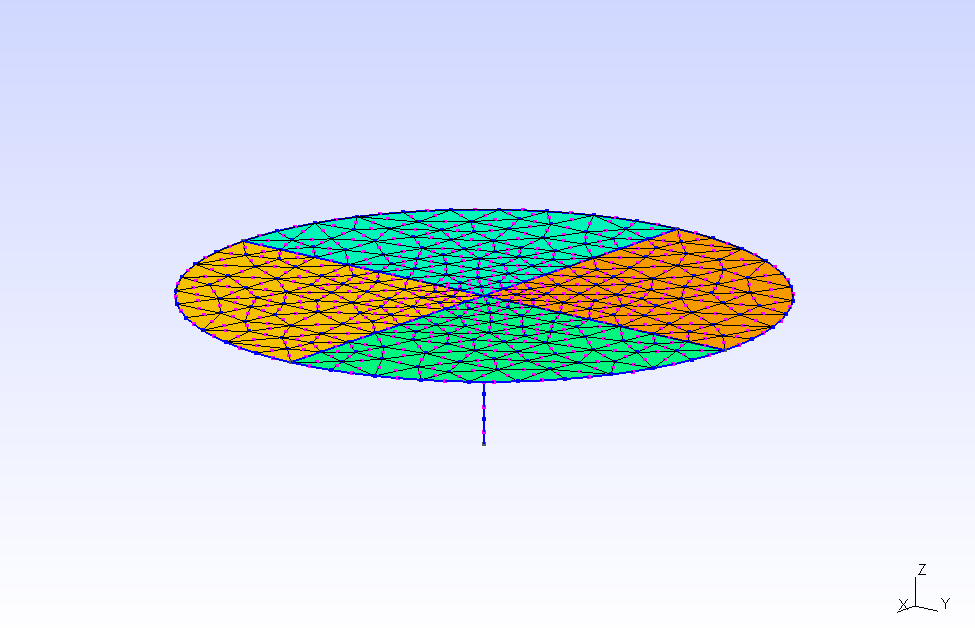
\includegraphics[scale = 0.58]{mesh.png}
	\caption{Mesh of the single battered pile resulting from the *.msh file.}
	\label{fig:mesh}
\end{figure}

\subsection{Input data file}
Solving in MultiFEBE consists of running the software by specifying several options in the following sections\footnote{See reference manual.}: [problem], [settings], [materials], [regions], [conditions over nodes], etc.

The first part to configurate is the problem definition in the section [problem]. This example is a 3D harmonic mechanical problem.

\begin{Verbatim}	
[problem]
n = 3D
type = mechanics
analysis = harmonic
\end{Verbatim}

Then, a list of frequencies is generated by specifying the number of frequencies, that must be $\geq 2$ (20) followed by the minimum frequency $>0$ (0.005976) and the maximum frequency (0.5976), being each one in new lines.

\begin{Verbatim}
[frequencies]
rad/s
lin
20
0.005976
0.5976
\end{Verbatim}

In the section [export], several export and notation settings are defined. In this example, the nodal solutions and the stress resultant solutions will be exported by writing the option F or T with the corresponding expression, ``export\_nso" and ``export\_tot", respectively. Furthermore, the complex notation is set as cartesian. 

\begin{Verbatim}
[export]
export_nso = T
export_tot = T
complex_notation = cartesian
\end{Verbatim}

As the problem has two materials, the section [materials] will need three lines: a first line for the number of materials in the model and a line per material with their properties such as tag, type, $\rho$, E, $\nu$ and $ \xi $.

\begin{Verbatim}
[materials]
2
1 elastic_solid rho 1. E 1. nu 0.4 xi 0.05
2 elastic_solid rho 0.428 E 1000. nu 0.25 xi 0.01
\end{Verbatim}

Next step is to configurate the mesh. In this case, a mesh from Gmsh will be used so that it is necessary to write the option number 2 and the document name obtained from it in the section [settings]. However, if the mesh were going to be read from the input file, it would require to write the sections [nodes], [elements] and [parts] instead.

\begin{Verbatim}	
[settings]
mesh_file_mode = 2 "single_pile.msh"
\end{Verbatim}

In the section [boundaries], all boundaries are defined. The first line indicates the number of boundaries (1). Then, one line per boundary indicating the boundary identifier (1), the part identifier that discretizes it (3), and finally the boundary class (ordinary).

\begin{Verbatim}
[boundaries]
1
1 3 ordinary
\end{Verbatim}

In the section [be body loads], all body loads in BE regions are defined. The format consists of a first line with the number of BE body loads to be defined, next as many lines as BE body loads. Each line contains first the BE body load identifier and last the mesh part which contains the elements associated with it.

\begin{Verbatim}
[be body loads]
1
1 1
\end{Verbatim}

The section [fe subregions] indicates the number of fe subregions in the first line (1) and a line per subregions indicating the subregion identifier (1) and the part identifier (2). The last two zeros at the end are mandatory and they are going to be used in the future for additional features.

\begin{Verbatim}
[fe subregions]
1
1 2 0 0
\end{Verbatim}

In the section [cross sections], it is necessary to specify the number of cross sections in the first line and a line per cross section by indicating the type of beam model (strbeam\_eb = straight beam, Euler–Bernoulli model), number of fe subregions related to the cross section (1), fe subregion identifier (1), type of cross section (circle), radius (1.) and reference vector for the section orientation (0. 1. 0.).

\begin{Verbatim}
[cross sections]
1
strbeam_eb 1 1 circle 1. 0. 1. 0.
\end{Verbatim}

The format of the section [regions] consists of a first line indicating the number of regions (2). Furthermore, for each region there must be a block of data consisting of several lines. 

The first region is a BE region, so the first line shows the region identifier and the region class (discretization method) (1 be). The second line indicates the number and list of boundaries (1 1), the third line defines the material (material 1), the fourth line defines the number and list of BE body loads (1 1) and the fifth line the number and list of incident fields (0).

The second region is a FE region, so the first line shows the region identifier and the region class (discretization method) (2 fe). Then, the second line indicates the number of subregions (1) and their identifiers (1) and the third line the material (material 2). 

\begin{Verbatim}	
[regions]
2

1 be
1 1
material 1
1 1
0

2 fe
1 1
material 2
\end{Verbatim}

In the section [groups], nodes and elements can be tagged depending on their position in space. The first line indicates the number of groups and then a line per group with the group tag and the command. In this example, a box is defined in space to select all the nodes inside it (nodes box interior) with its maximum and minimum x, y and z coordinates (-0.001 0.001 -0.001 0.001 -0.001 0.001), respectively, and the part where the nodes belong (2).    

\begin{Verbatim}
[groups]
1
1 nodes box interior -0.001 0.001 -0.001 0.001 -0.001 0.001 2 
\end{Verbatim}

In the section [conditions over nodes], all boundary conditions over nodes or groups will be specified. As a 3D model, there are 6 lines for every boundary condition. Every line has two digits, where the first one indicates the type of condition (0 for displacement and 1 for force) and the second one the value in complex number (real part, imaginary part) because it is a harmonic analysis. In case of displacement, firstly the displacements $u_x, u_y, u_z$ are configured and then the rotations $\theta_x, \theta_y, \theta_z$. In case of force, firstly the forces $F_x, F_y, F_z$ and then the moments $M_x, M_y, M_z$. 

\begin{Verbatim}	
[conditions over nodes]
group 1: 0 (1.,0.)
         0 (0.,0.)
         0 (0.,0.)
         0 (0.,0.)
         0 (0.,0.)
         0 (0.,0.)
\end{Verbatim}

The whole data file applied to the problem is the following:

\begin{Verbatim}
[problem]
n = 3D
type = mechanics
analysis = harmonic

[frequencies]
rad/s
lin
20
0.005976
0.5976

[export]
export_nso = T
export_tot = T
complex_notation = cartesian

[materials]
2
1 elastic_solid rho 1. E 1. nu 0.4 xi 0.05
2 elastic_solid rho 0.428 E 1000. nu 0.25 xi 0.01

[settings]
mesh_file_mode = 2 "single_pile.msh"

[boundaries]
1
1 3 ordinary

[be body loads]
1
1 1

[fe subregions]
1
1 2 0 0

[cross sections]
1
strbeam_eb 1 1 circle 1. 0. 1. 0.

[regions]
2
1 be
1 1
material 1
1 1
0

2 fe
1 1
material 2

[groups]
1
1 nodes box interior -0.001 0.001 -0.001 0.001 -0.001 0.001 2 

[conditions over nodes]
group 1: 0 (1.,0.)
         0 (0.,0.)
         0 (0.,0.)
         0 (0.,0.)
         0 (0.,0.)
         0 (0.,0.)
\end{Verbatim}

\subsection{Results and discussion}

Figures \ref{fig:khh}, \ref{fig:khr} and \ref{fig:krr} show the horizontal, horizontal–rocking crossed and rocking impedances for a single battered pile with different angles of inclination. The results from \cite{giannakou}, \cite{poulos} and \cite{padron} are shown together with the obtained results from the present model. It is observed a very good agreement. 

\begin{figure}[tbh!]
	\centering
	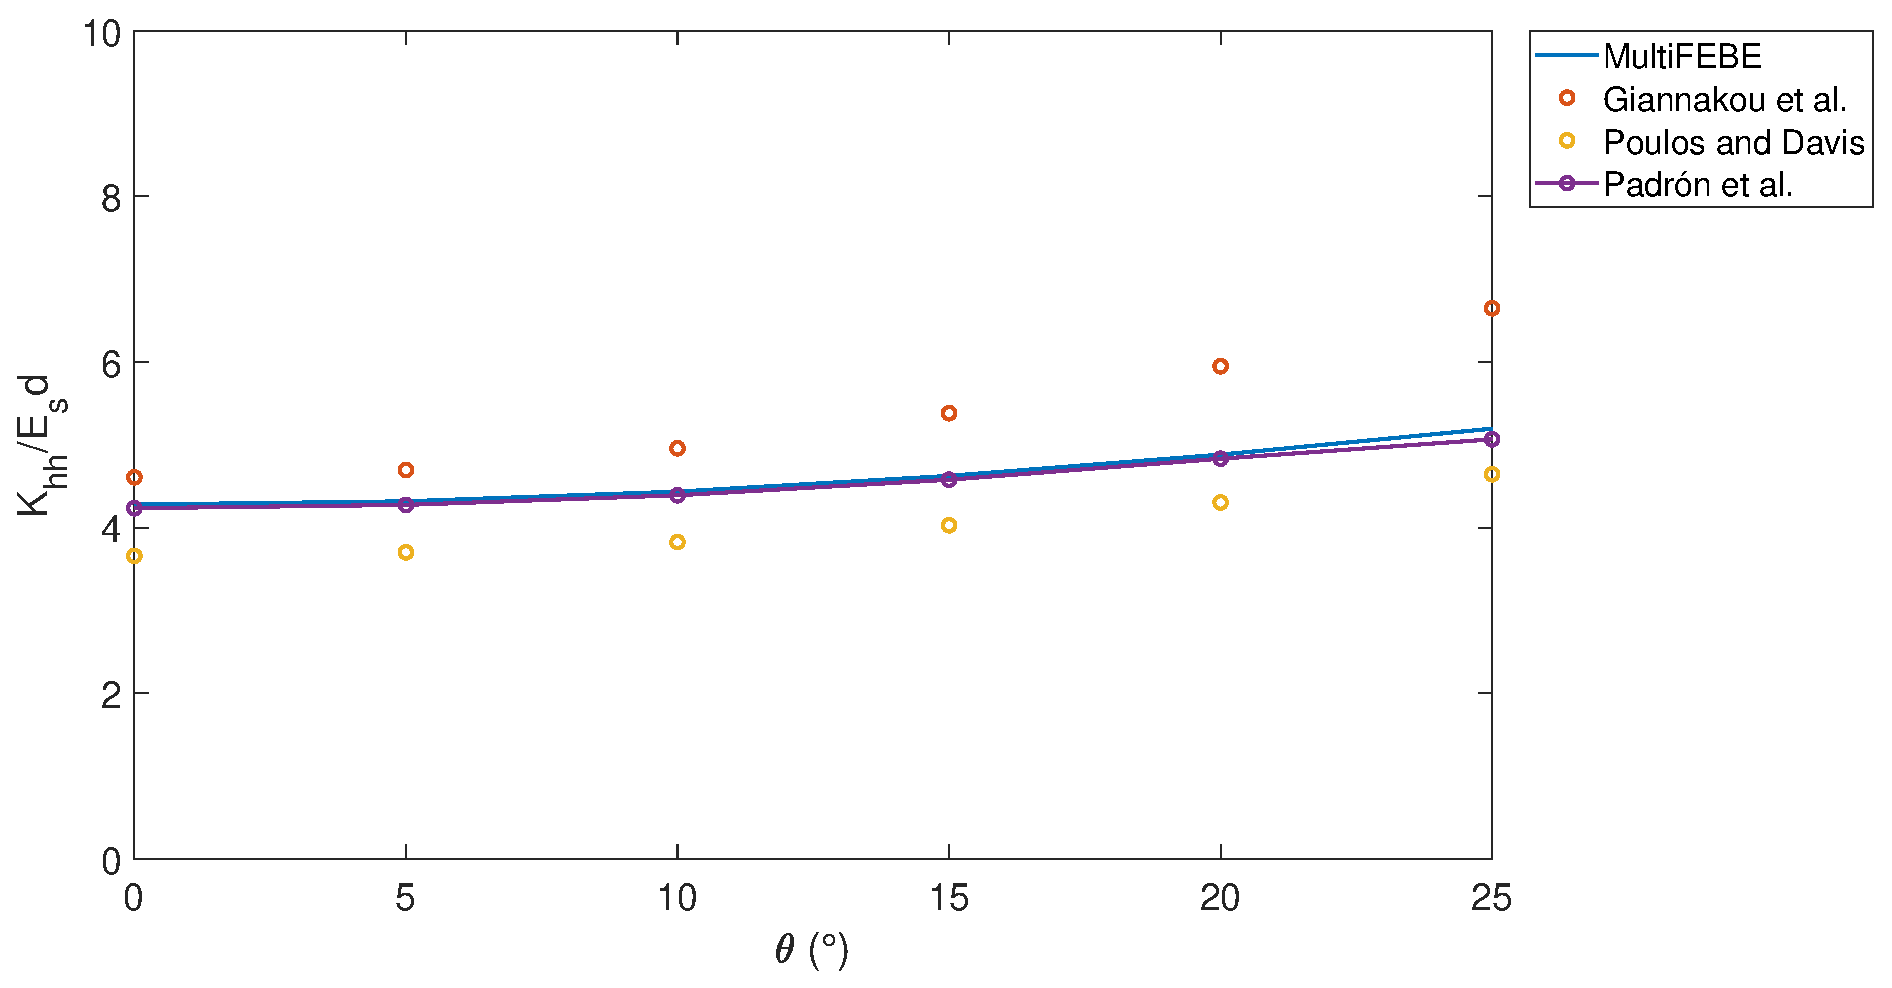
\includegraphics[scale=0.5]{khh.eps}
	\caption{Horizontal impedance.}
	\label{fig:khh}
\end{figure}

\begin{figure}[tbh!]
	\centering
	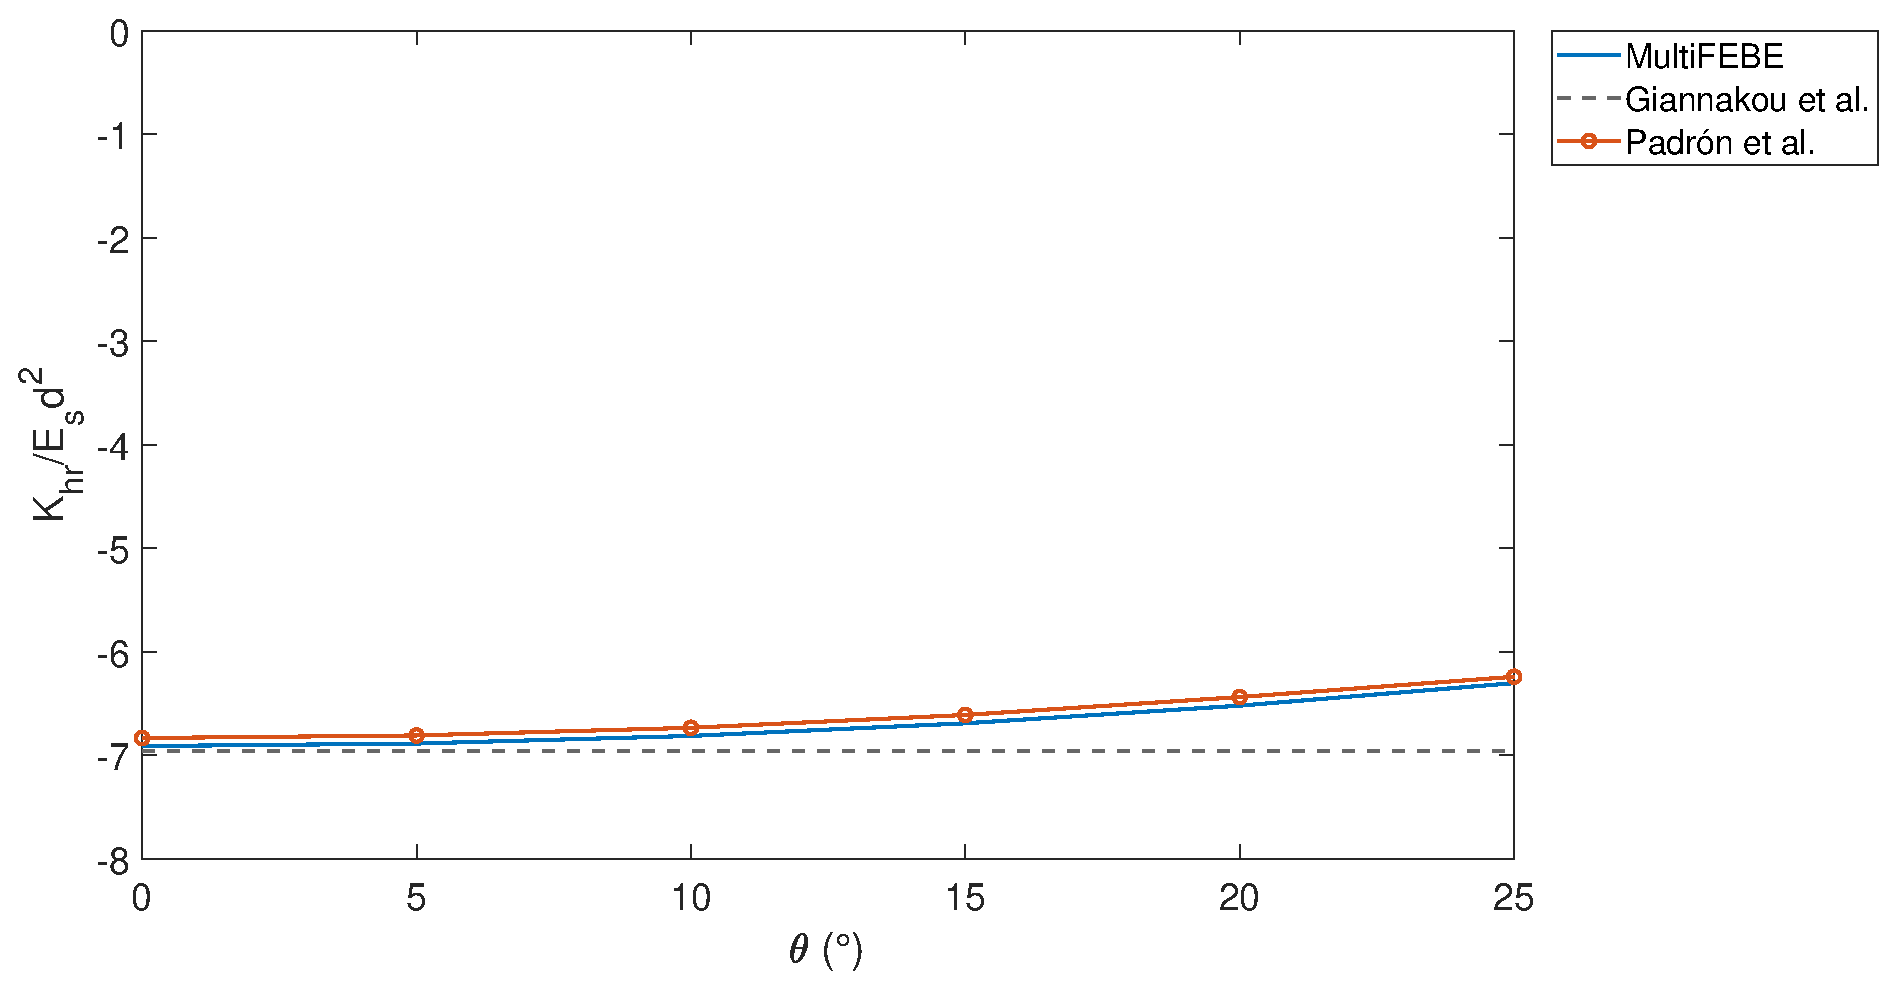
\includegraphics[scale=0.5]{khr.eps}
	\caption{Horizontal–rocking crossed impedance.}
	\label{fig:khr}
\end{figure}

\begin{figure}[tbh!]
	\centering
	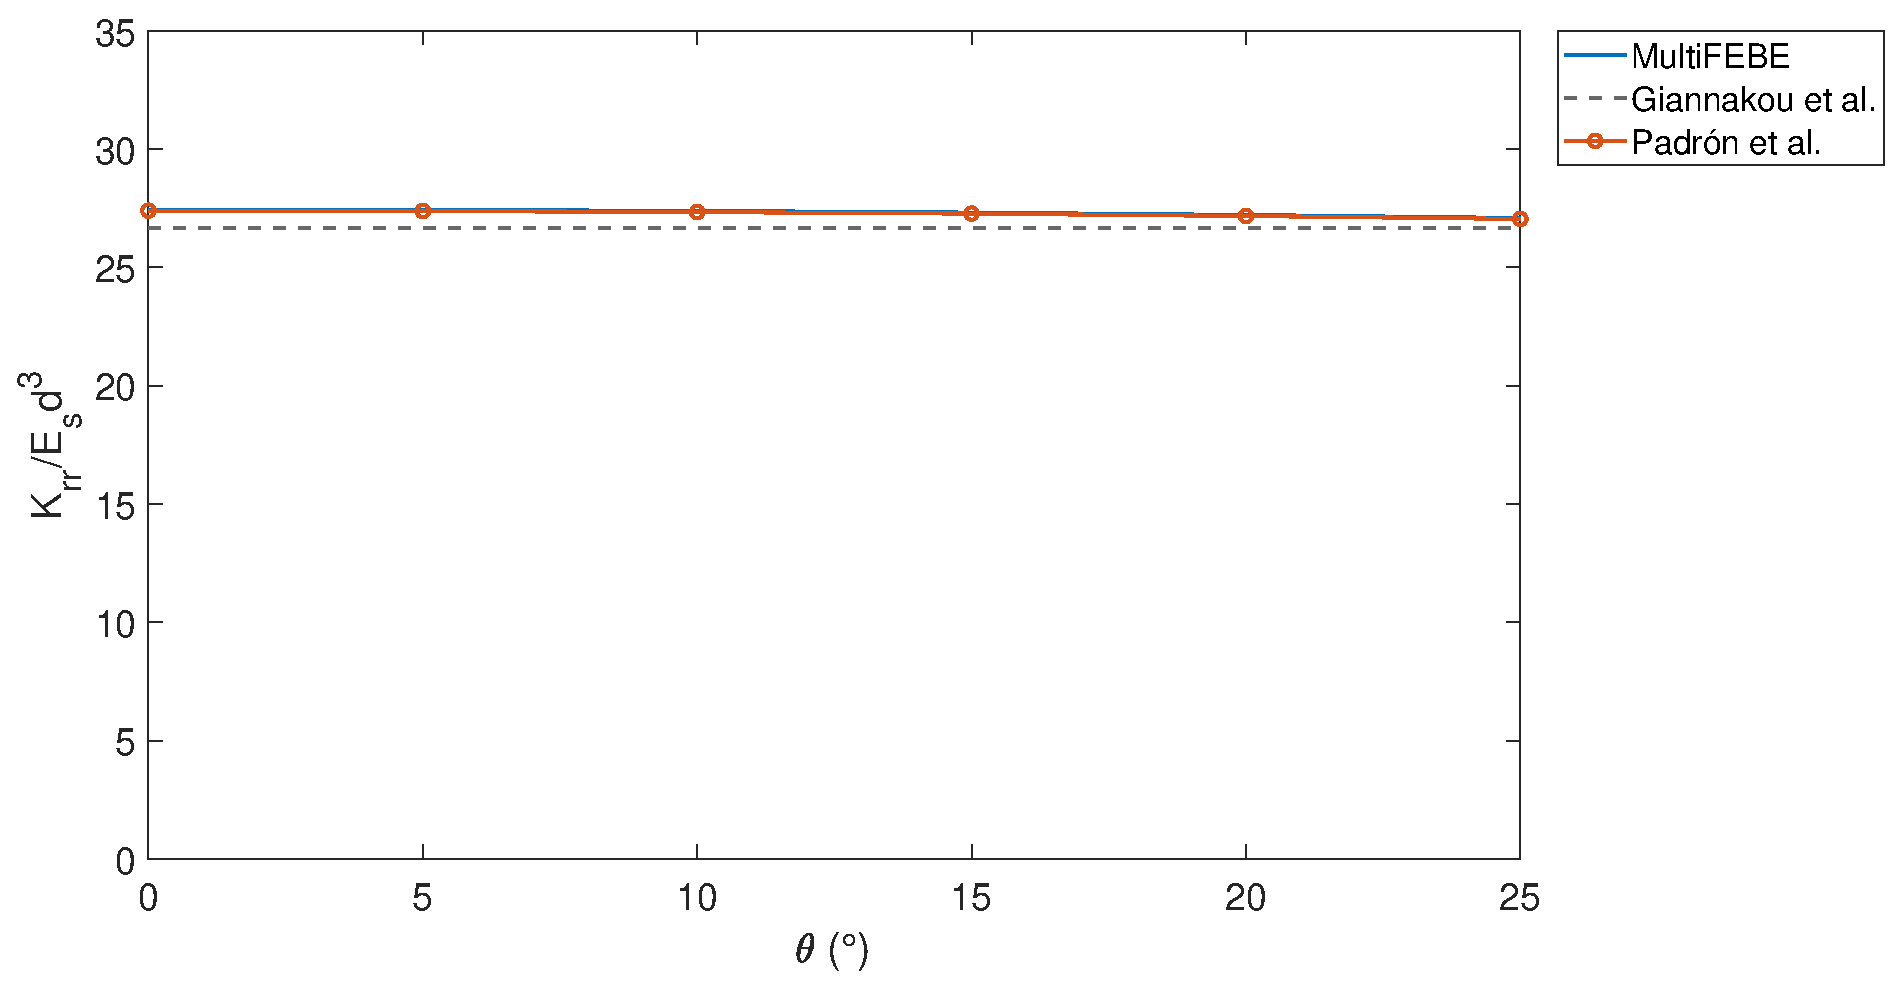
\includegraphics[scale=0.5]{krr.eps}
	\caption{Rocking impedance.}
	\label{fig:krr}
\end{figure}

\section{$2 \times 2 $ pile group with battered elements}

In this section, the horizontal, horizontal–rocking crossed and rocking impedances of a $2 \times 2 $ group of piles will be calculated by subjecting pile heads to forced vibration in each of the oscillation modes. This process will be done from the proper combination of the contributions of each pile for an angle of 20° between the pile axis and the vertical \cite{padron}.

First of all, the whole model will be simulated and then the quarter symmetric model.

\subsection{Whole model}

\subsubsection{GEO file}

\begin{Verbatim}
// Geometry & mesh parameters
D = 1;
L = 15;
s_D = 5; // Ratio pile separation - diameter
theta = -20;
ms_pile = 2.5;
ms_near = 1.5;
ms_far = 3;
R_truncation = 2.5*L;

theta = theta*Pi/180; 
xp = s_D/2;           
yp = s_D/2;           

Point (1) = {xp,yp,0,ms_pile};
Point (2) = {xp-L*Sin(theta),2.5,-L*Cos(theta),ms_pile};
Line  (1) = {1,2};
Transfinite Line{1}=Round(L/ms_pile+1.);
Physical Line ("line-load_1") = {1};

Point (3) = {xp,yp,0,ms_pile};
Point (4) = {xp-L*Sin(theta),2.5,-L*Cos(theta),ms_pile};
Line  (2) = {3,4};
Transfinite Line{2}=Round(L/ms_pile+1.);
Physical Line ("pile_1") = {2};

Point (5) = {xp,-yp,0,ms_pile};
Point (6) = {xp-L*Sin(theta),-2.5,-L*Cos(theta),ms_pile};
Line  (3) = {5,6};
Transfinite Line{3}=Round(L/ms_pile+1.);
Physical Line ("line-load_2") = {3};

Point (7) = {xp,-yp,0,ms_pile};
Point (8) = {xp-L*Sin(theta),-2.5,-L*Cos(theta),ms_pile};
Line  (4) = {7,8};
Transfinite Line{4}=Round(L/ms_pile+1.);
Physical Line ("pile_2") = {4};

Point (9) = {-xp,-yp,0,ms_pile};
Point (10) = {-xp-L*Sin(-theta),-2.5,-L*Cos(-theta),ms_pile};
Line  (5) = {9,10};
Transfinite Line{5}=Round(L/ms_pile+1.);
Physical Line ("line-load_3") = {5};

Point (11) = {-xp,-yp,0,ms_pile};
Point (12) = {-xp-L*Sin(-theta),-2.5,-L*Cos(-theta),ms_pile};
Line  (6) = {11,12};
Transfinite Line{6}=Round(L/ms_pile+1.);
Physical Line ("pile_3") = {6};

Point (13) = {-xp,yp,0,ms_pile};
Point (14) = {-xp-L*Sin(-theta),2.5,-L*Cos(-theta),ms_pile};
Line  (7) = {13,14};
Transfinite Line{7}=Round(L/ms_pile+1.);
Physical Line ("line-load_4") = {7};

Point (15) = {-xp,yp,0,ms_pile};
Point (16) = {-xp-L*Sin(-theta),2.5,-L*Cos(-theta),ms_pile};
Line  (8) = {15,16};
Transfinite Line{4}=Round(L/ms_pile+1.);
Physical Line ("pile_4") = {8};

Point (17) = {            0 ,            0 , 0 , ms_near };
Point (18) = { R_truncation ,            0 , 0 , ms_far };
Point (19) = {            0 , R_truncation , 0 , ms_far };
Point (20) = {-R_truncation ,            0 , 0 , ms_far };
Point (21) = {            0, -R_truncation , 0 , ms_far };

Line  (9) = {17,18};
Circle(10) = {18,17,19};
Line  (11) = {19,17};
Line Loop (12) = {9,10,11}; 
Plane Surface(1) = {12};

Line  (13) = {20,17};
Circle(14) = {19,17,20};
Line Loop (15) = {13,-11,14}; 
Plane Surface(2) = {15};

Line  (16) = {21,17};
Circle(17) = {20,17,21};
Line Loop (18) = {16,-13,17}; 
Plane Surface(3) = {18};

Circle(19) = {21,17,18};
Line Loop (20) = {-16,19,-9}; 
Plane Surface(4) = {20};

// Embedding points in the surfaces 
Point (22) = {xp,yp,0,ms_near};
Point (23) = {xp,-yp,0,ms_near};
Point (24) = {-xp,-yp,0,ms_near};
Point (25) = {-xp,yp,0,ms_near};
Point {22} In Surface {1};
Point {23} In Surface {2};
Point {24} In Surface {3};
Point {25} In Surface {4};

Physical Surface("free-surface") = {1,2,3,4};

// Mesh generation
Mesh 2;
SetOrder 2;
Save "whole_group.msh";
\end{Verbatim}

\begin{figure}[tbh!]
	\centering
	\begin{subfigure}[b]{0.48\textwidth}
		\centering
		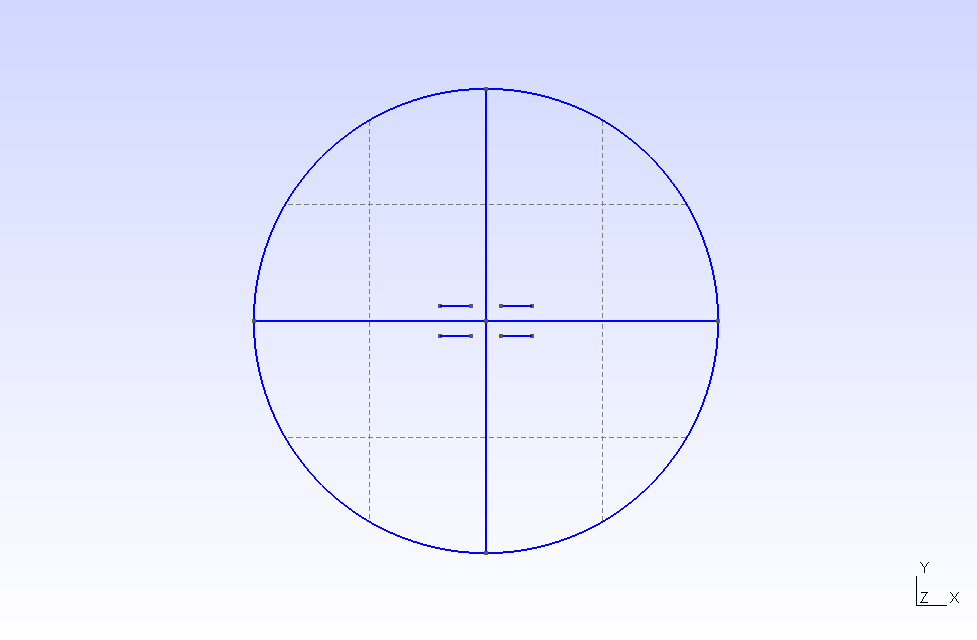
\includegraphics[width=\textwidth]{geometry_whole1.png}
		\caption{Top view of the whole model.}
		\label{fig:geometry_whole1}
	\end{subfigure}
	\begin{subfigure}[b]{0.48\textwidth}
		\centering
		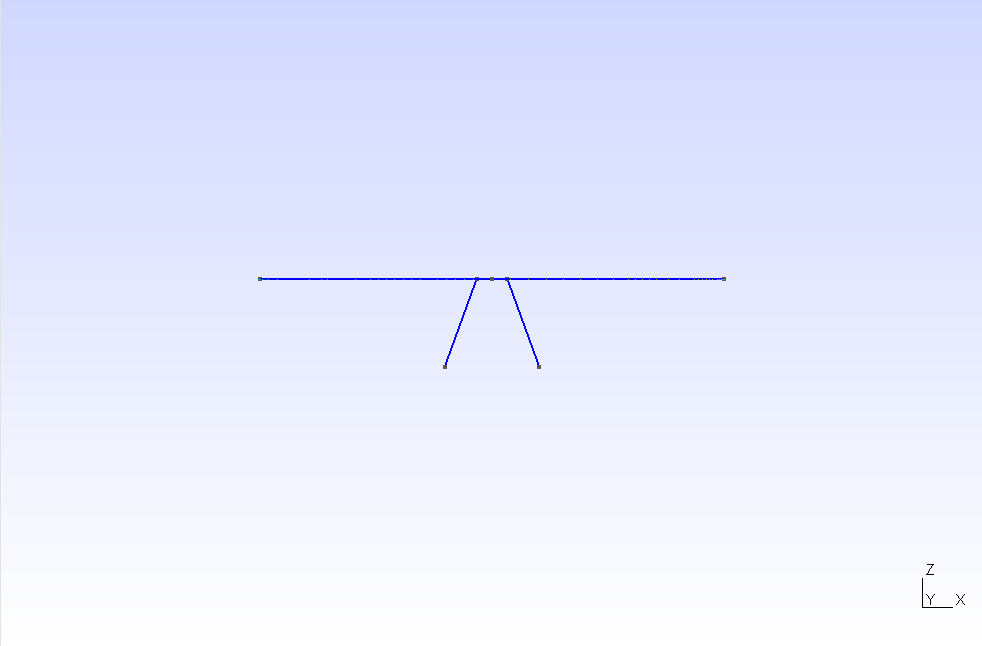
\includegraphics[width=\textwidth]{geometry_whole2.png}
		\caption{Side view of the whole model.}
		\label{fig:geometry_whole2}
	\end{subfigure}
	\caption{Geometry of the whole model resulting from the *.geo file.}
\label{fig:geometry_2x2_group}
\end{figure}

\begin{figure}[tbh!]
	\centering
	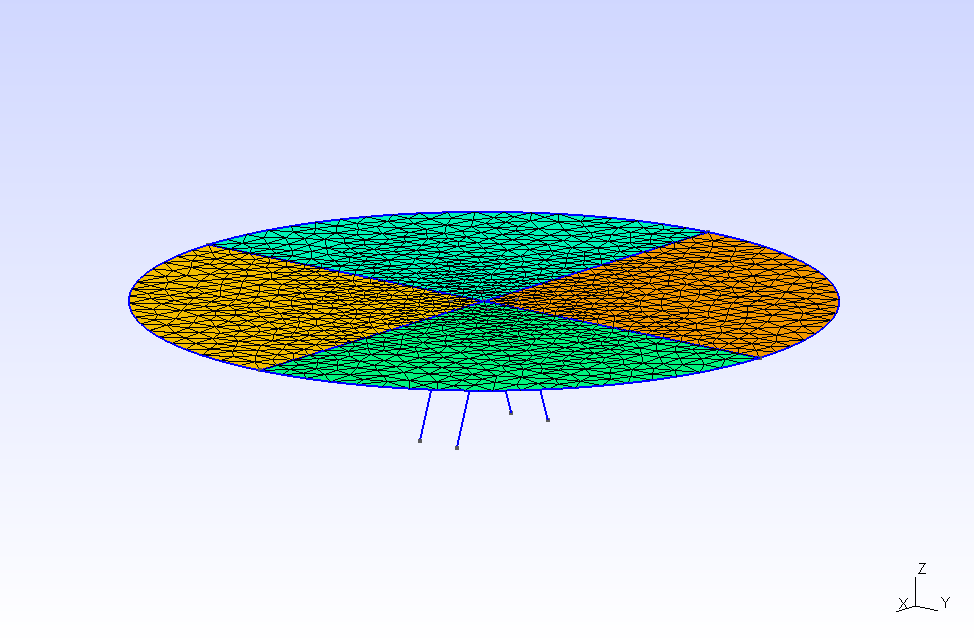
\includegraphics[scale=0.58]{mesh_whole.png}
	\caption{Mesh of the whole model resulting from the *.msh file.}
	\label{fig:mesh_whole}
\end{figure}

\subsubsection{Input data file}

\begin{Verbatim}
[problem]
n = 3D
type = mechanics
analysis = harmonic

[frequencies]
rad/s
lin
20
0.005976
0.5976

[export]
export_nso = T
export_tot = T
complex_notation = cartesian

[materials]
2
1 elastic_solid rho 1. E 1. nu 0.4 xi 0.05
2 elastic_solid rho 0.428 E 1000. nu 0.25 xi 0.01

[settings]
mesh_file_mode = 2 "whole_group.msh"

[boundaries]
1
1 9 ordinary

[be body loads]
4
1 1
2 3
3 5
4 7

[fe subregions]
4
1 2 0 0
2 4 0 0
3 6 0 0
4 8 0 0

[cross sections]
1
strbeam_eb 4 1 2 3 4 circle 1. 0. 1. 0.

[regions]
2
1 be
1 1
material 1
4 1 2 3 4
0

2 fe
4 1 2 3 4
material 2

[conditions over nodes]
node 3: 0 (1.,0.)
        0 (0.,0.)
        0 (0.,0.)
        0 (0.,0.)
        0 (0.,0.)
        0 (0.,0.)

node 7: 0 (1.,0.)
        0 (0.,0.)
        0 (0.,0.)
        0 (0.,0.)
        0 (0.,0.)
        0 (0.,0.)

node 11: 0 (1.,0.)
         0 (0.,0.)
         0 (0.,0.)
         0 (0.,0.)
         0 (0.,0.)
         0 (0.,0.)

node 15: 0 (1.,0.)
         0 (0.,0.)
         0 (0.,0.)
         0 (0.,0.)
         0 (0.,0.)
         0 (0.,0.)
\end{Verbatim}

\subsection{Symmetric quarter model}

\subsubsection{GEO file}

\begin{Verbatim}
// Geometry & mesh parameters
D = 1;
L = 15;
s_D = 5; 
theta = -20;  
ms_pile = 2.5;
ms_near = 1.5;
ms_far = 3;
R_truncation = 2.5*L;

theta = theta*Pi/180; 
xp = s_D/2;           
yp = s_D/2;           

Point (1) = {xp,yp,0,ms_pile};                          
Point (2) = {xp-L*Sin(theta),yp,-L*Cos(theta),ms_pile}; 
Line  (1) = {1,2};
Transfinite Line{1}=Round(L/ms_pile+1.);
Physical Line ("line-load_1") = {1};

Point (3) = {xp,yp,0,ms_pile};                           
Point (4) = {xp-L*Sin(theta),yp,-L*Cos(theta),ms_pile};   
Line  (2) = {3,4};
Transfinite Line{2}=Round(L/ms_pile+1.);
Physical Line ("pile_1") = {2};

Point (17) = {            0 ,            0 , 0 , ms_near };
Point (18) = { R_truncation ,            0 , 0 , ms_far };
Point (19) = {            0 , R_truncation , 0 , ms_far };

Line  (9) = {17,18};
Circle(10) = {18,17,19};
Line  (11) = {19,17};
Line Loop (12) = {9,10,11}; 
Plane Surface(1) = {12};

// Embedding a point in the surface 
Point (20) = {xp,yp,0,ms_near};  
Point {20} In Surface {1};

Physical Surface("free-surface") = {1};

// Mesh generation
Mesh 2;
SetOrder 2;
Save "symmetric_quarter_group.msh";
\end{Verbatim}

\begin{figure}[tbh!]
	\centering
	\begin{subfigure}[b]{0.48\textwidth}
		\centering
		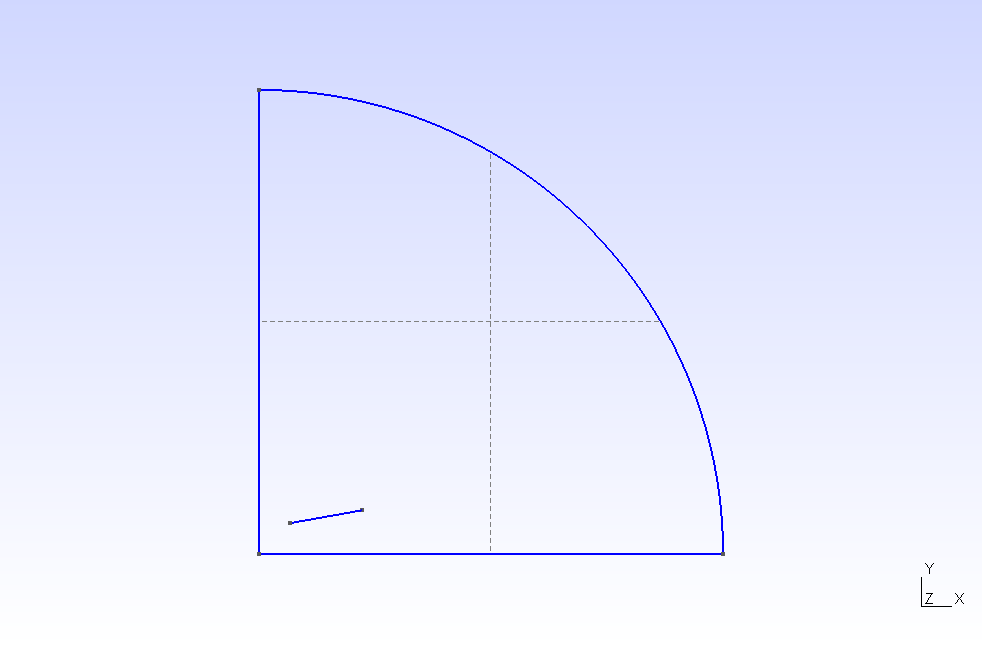
\includegraphics[width=\textwidth]{geometry_quarter1.png}
		\caption{Top view of the symmetric quarter model.}
		\label{fig:geometry_quarter1}
	\end{subfigure}
	\begin{subfigure}[b]{0.48\textwidth}
		\centering
		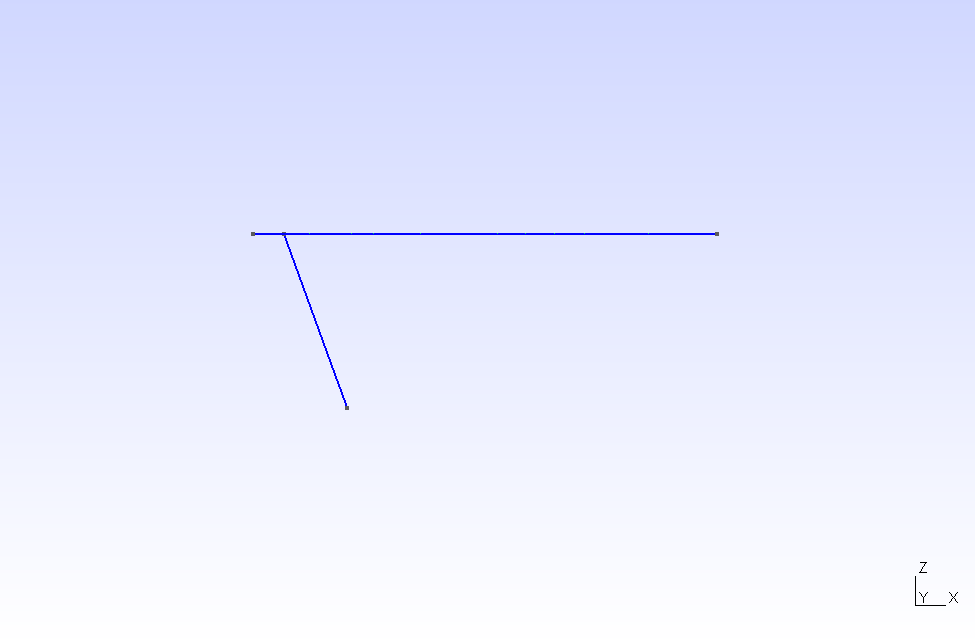
\includegraphics[width=\textwidth]{geometry_quarter2.png}
		\caption{Side view of the Symmetric quarte model.}
		\label{fig:geometry_quarter2}
	\end{subfigure}
	\caption{Geometry of the symmetric quarter model resulting from the *.geo file.}
\label{fig:geometry_symmetric_2x2_group}
\end{figure}

\begin{figure}[tbh!]
	\centering
	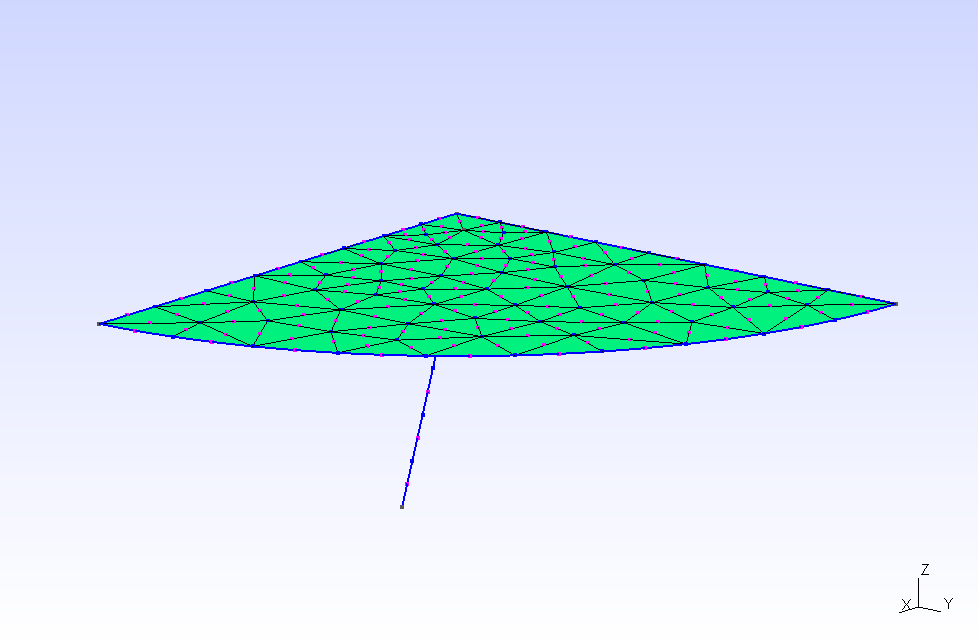
\includegraphics[scale=0.58]{mesh_quarter.png}
	\caption{Mesh of the symmetric quarter model resulting from the  *.msh file.}
	\label{fig:mesh_quarter}
\end{figure}

\subsubsection{Input data file}

\begin{Verbatim}
[problem]
n = 3D
type = mechanics
analysis = harmonic

[frequencies]
rad/s
lin
20
0.005976
0.5976

[export]
export_nso = T
export_tot = T
complex_notation = cartesian

[materials]
2
1 elastic_solid rho 1. E 1. nu 0.4 xi 0.05
2 elastic_solid rho 0.428 E 1000. nu 0.25 xi 0.01

[settings]
mesh_file_mode = 2 "symmetric_quarter_group.msh"

[boundaries]
1
1 3 ordinary

[be body loads]
1
1 1

[fe subregions]
1
1 2 0 0

[cross sections]
1
strbeam_eb 1 1 circle 1. 0. 1. 0.

[regions]
2
1 be
1 1
material 1
1 1
0

2 fe
1 1
material 2

[symmetry planes]
plane_n1: antisymmetry
plane_n2: symmetry

[conditions over nodes]
node 3:  0 (1.,0.)
         0 (0.,0.)
         0 (0.,0.)
         0 (0.,0.)
         0 (0.,0.)
         0 (0.,0.)
\end{Verbatim}

\subsection{Results and discussion}

Figures \ref{fig:khh_2x2_group}, \ref{fig:chh_2x2_group}, \ref{fig:krh_2x2_group}, \ref{fig:crh_2x2_group}, \ref{fig:krr_2x2_group} and \ref{fig:crr_2x2_group} show the horizontal, horizontal–rocking crossed and rocking impedances for a $2 \times 2 $ pile group with an angle of inclination of 20°. The results from \cite{padron} are shown together with the results from the whole model and the symmetric quarter model. It is observed a very good agreement between the whole and the symmetric model and small discrepancies (more acute in krh and crh) with respect to Padrón \textit{et al.}, presumably due to the difference in the size mesh and area of the free surface and due to the fact that the results from \cite{padron} have load on tip, but the results from MultiFEBE don't. 

\begin{figure}[h!]
	\centering
	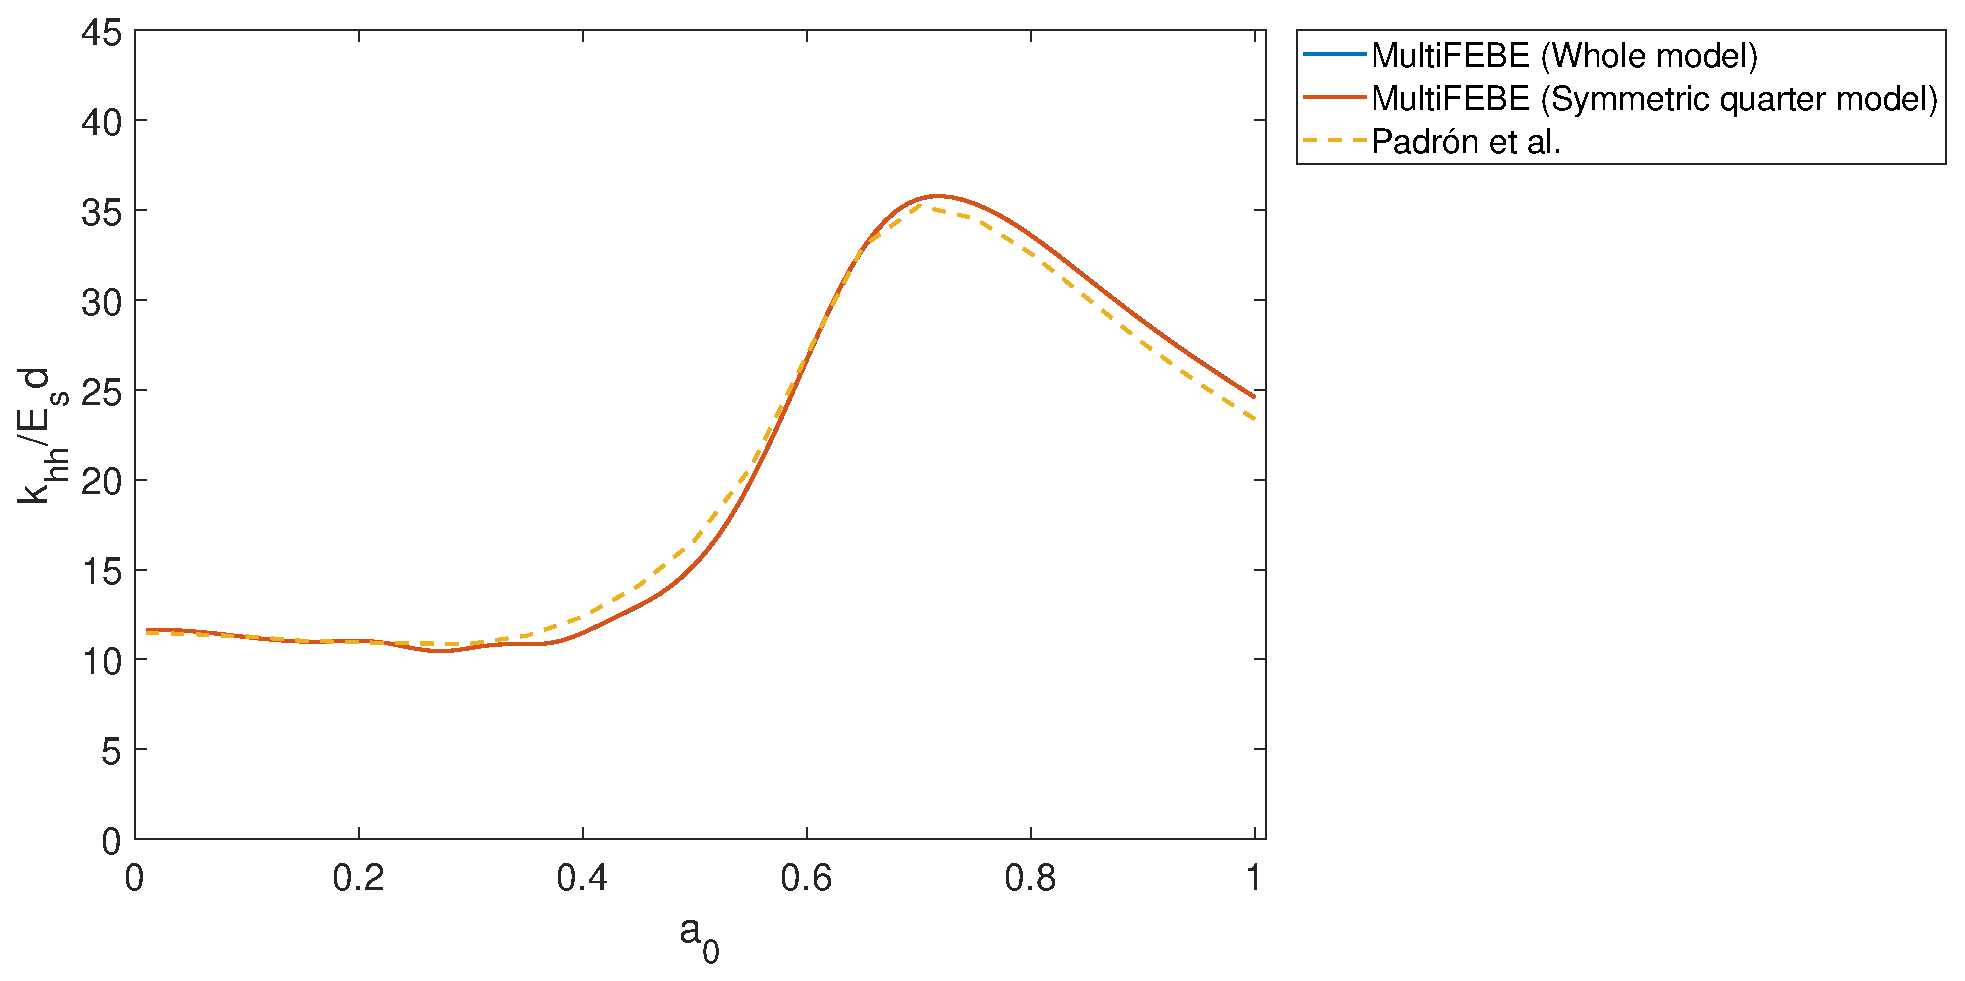
\includegraphics[scale=0.5]{khh_2x2_group.eps}
	\caption{Horizontal impedance (khh).}
	\label{fig:khh_2x2_group}
\end{figure}

\begin{figure}[h!]
	\centering
	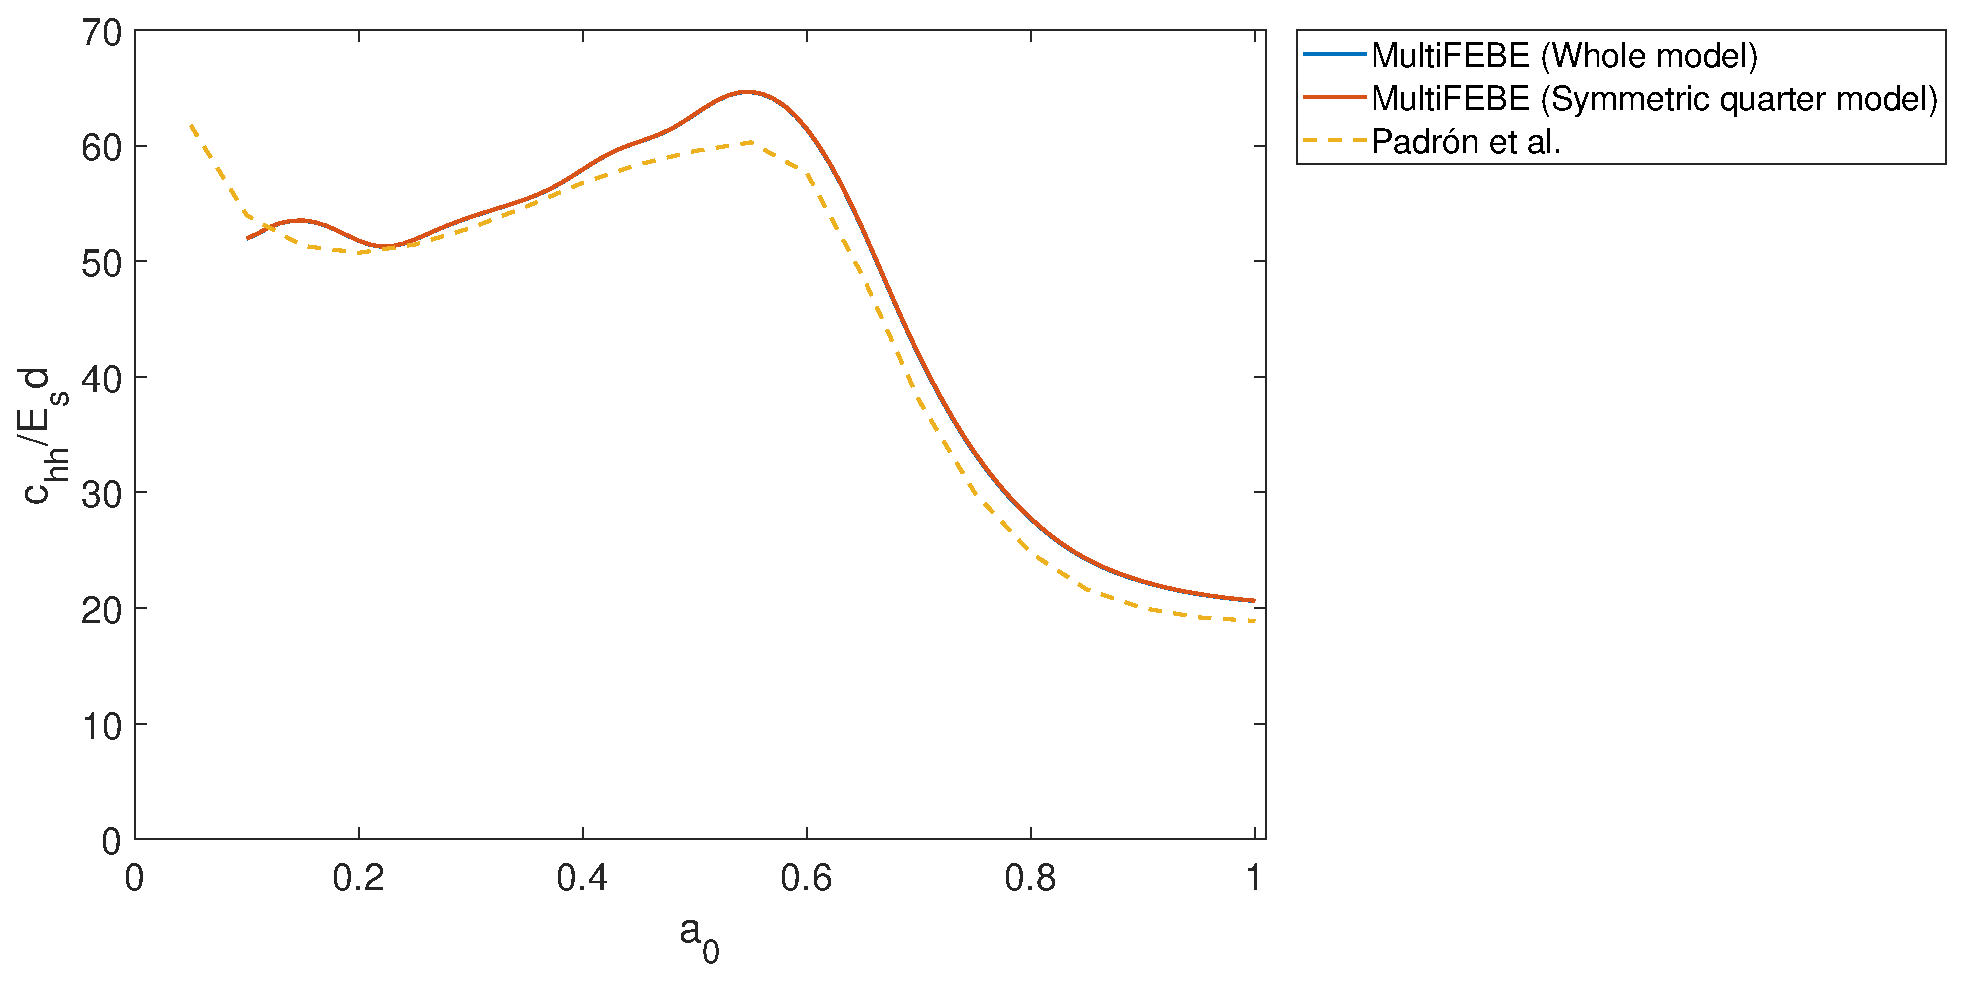
\includegraphics[scale=0.5]{chh_2x2_group.eps}
	\caption{Horizontal impedance (chh).}
	\label{fig:chh_2x2_group}
\end{figure}

\begin{figure}[h!]
	\centering
	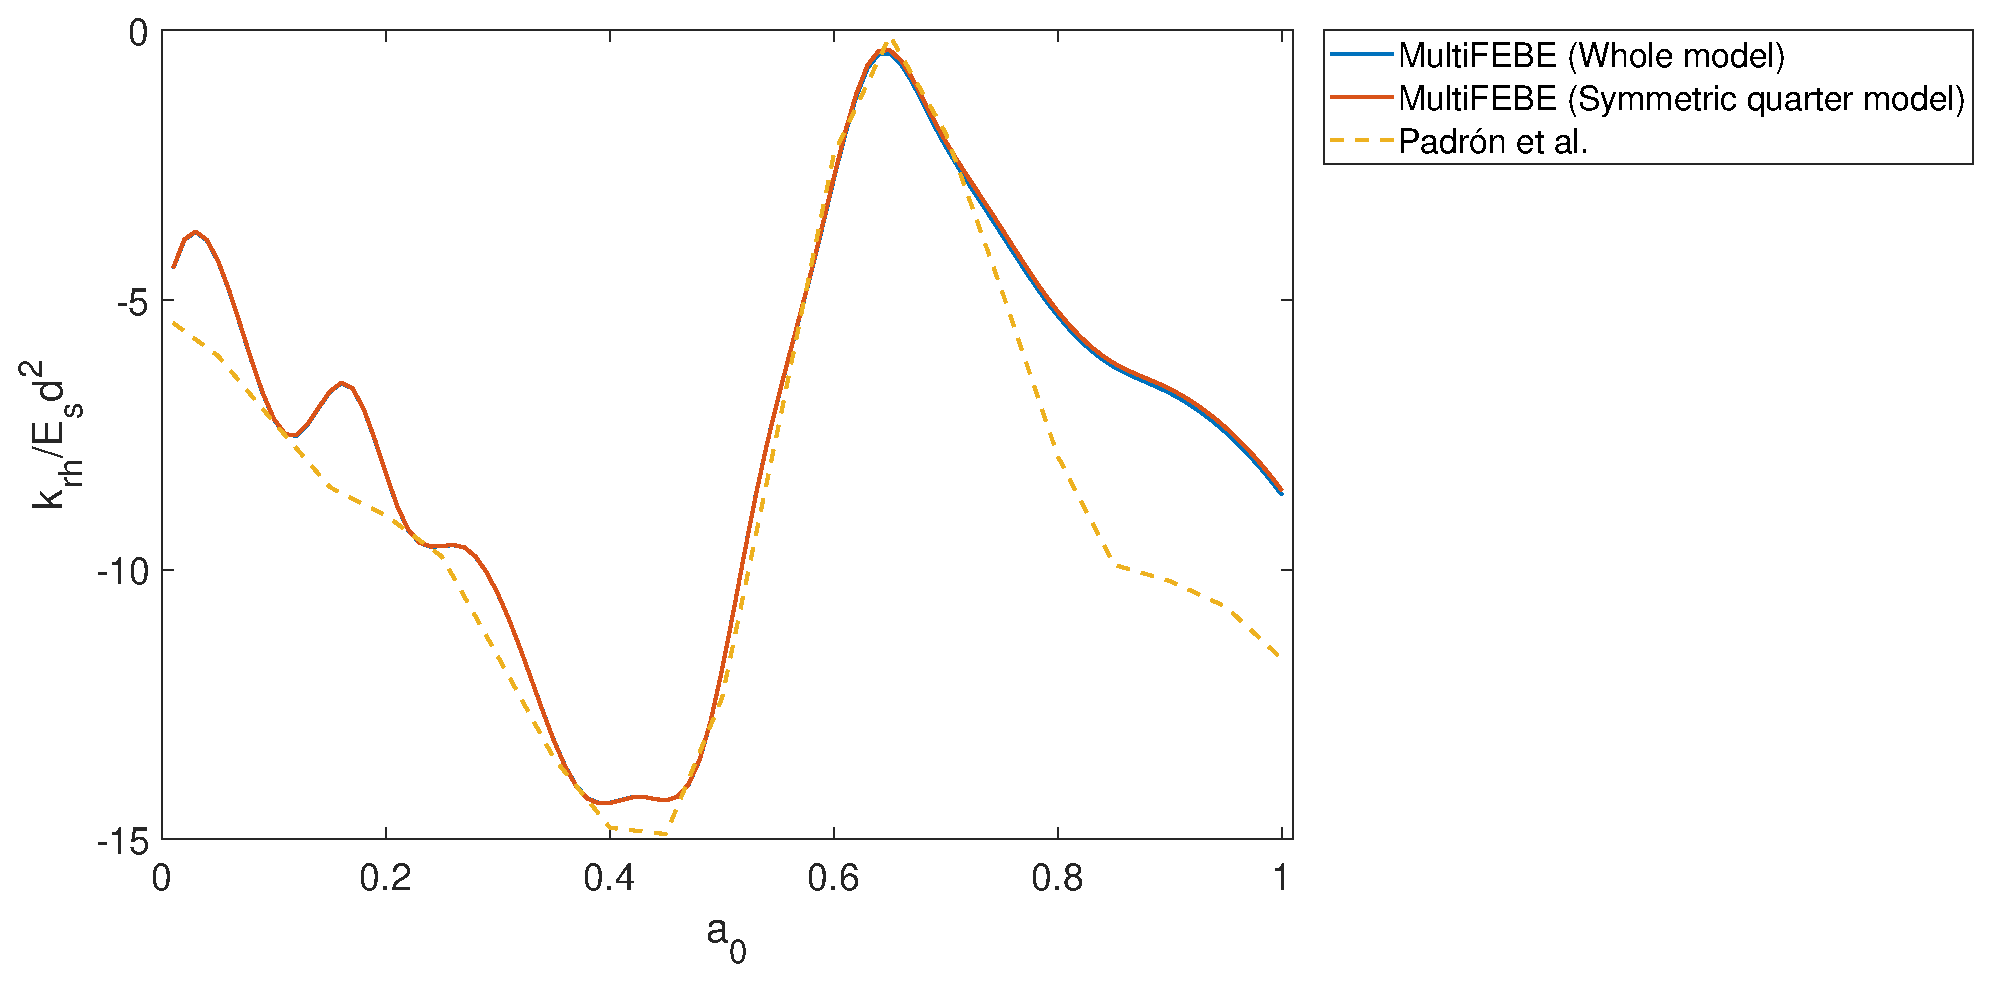
\includegraphics[scale=0.5]{krh_2x2_group.eps}
	\caption{Horizontal–rocking crossed impedance (krh).}
	\label{fig:krh_2x2_group}
\end{figure}

\begin{figure}[h!]
	\centering
	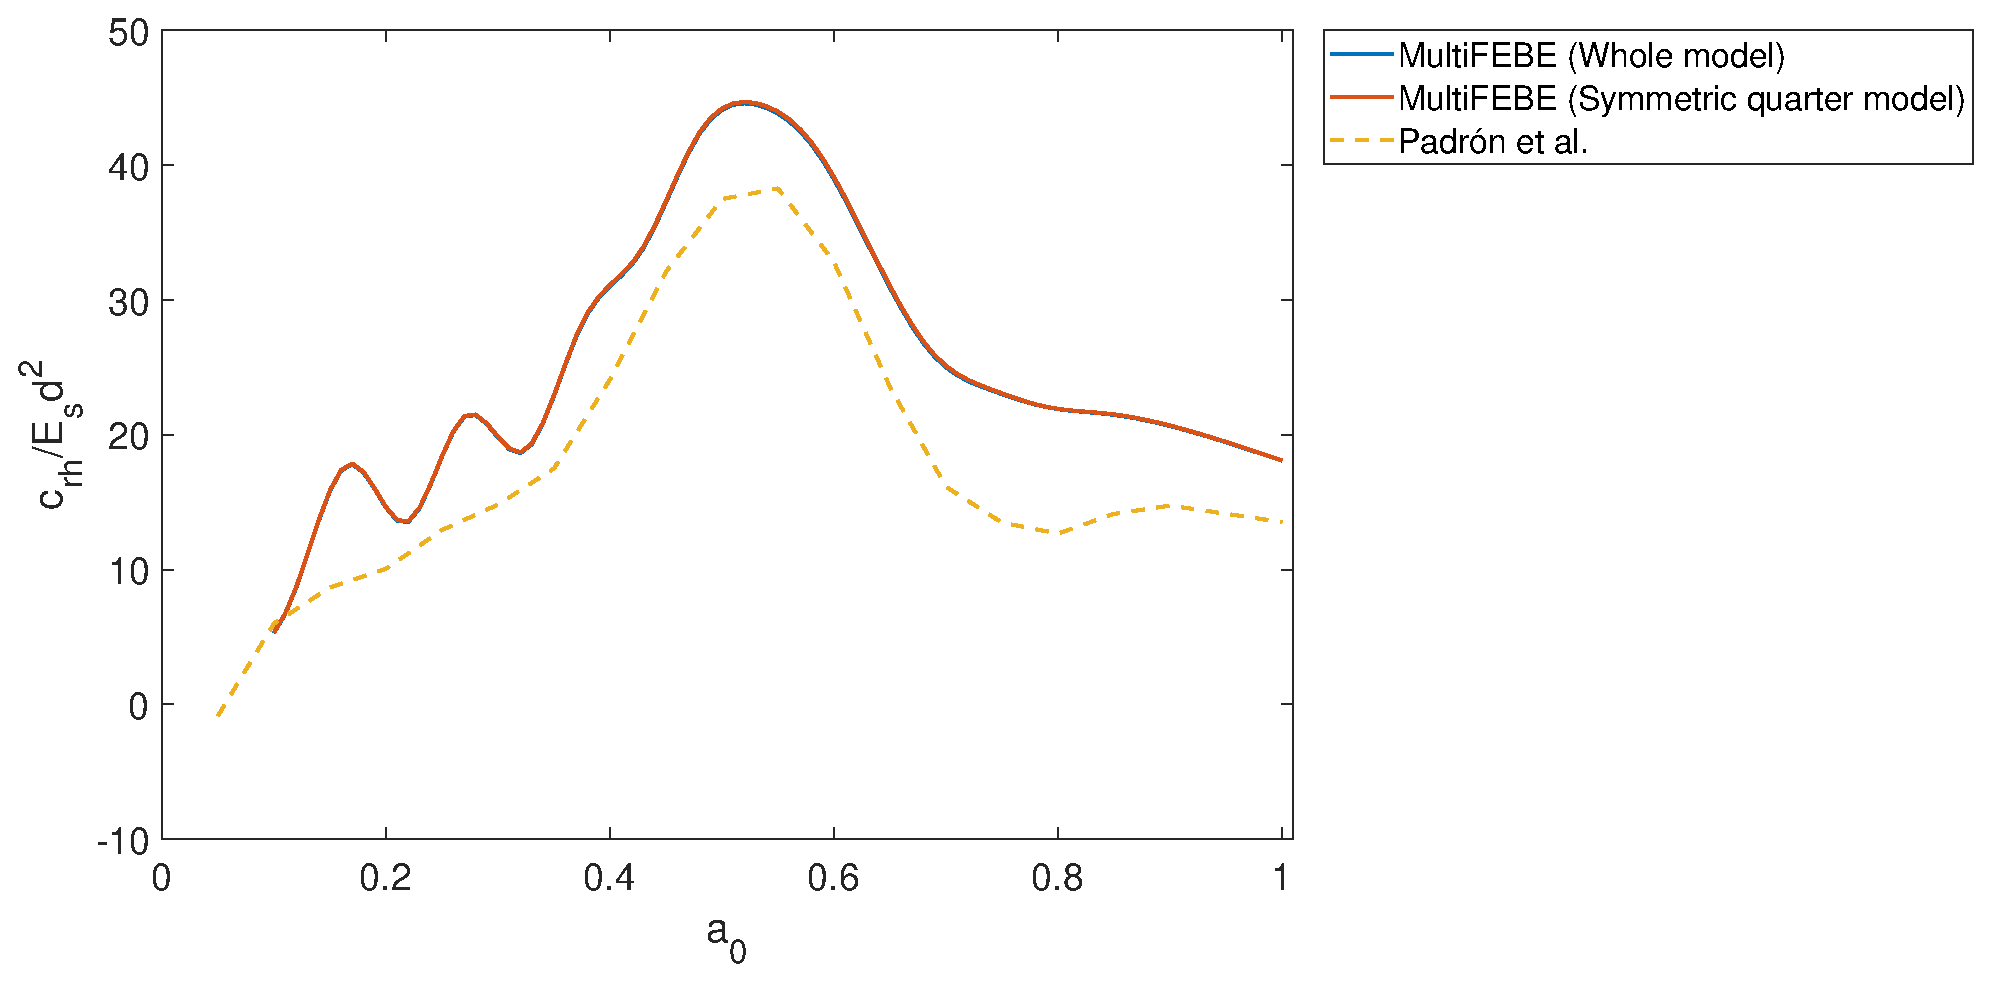
\includegraphics[scale=0.5]{crh_2x2_group.eps}
	\caption{Horizontal–rocking crossed impedance (crh).}
	\label{fig:crh_2x2_group}
\end{figure}

\begin{figure}[h!]
	\centering
	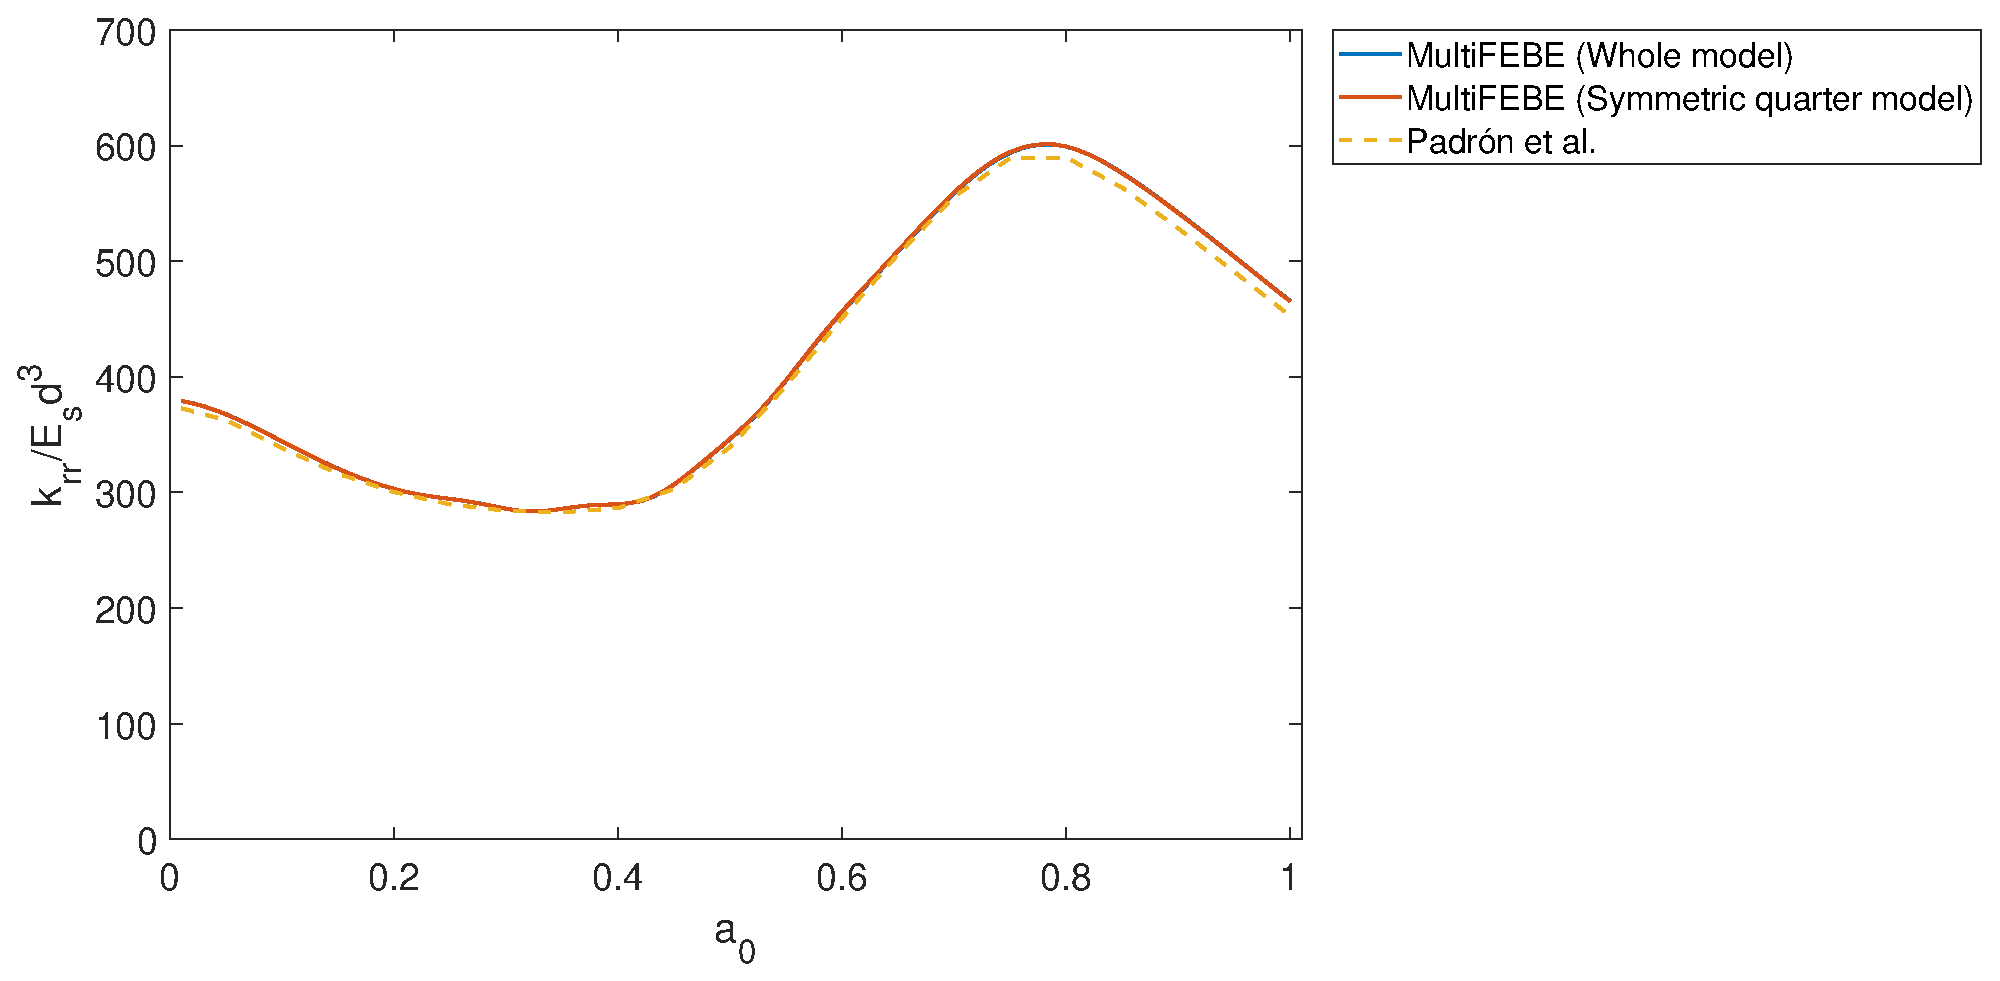
\includegraphics[scale=0.5]{krr_2x2_group.eps}
	\caption{Rocking impedance (krr).}
	\label{fig:krr_2x2_group}
\end{figure}

\begin{figure}[h!]
	\centering
	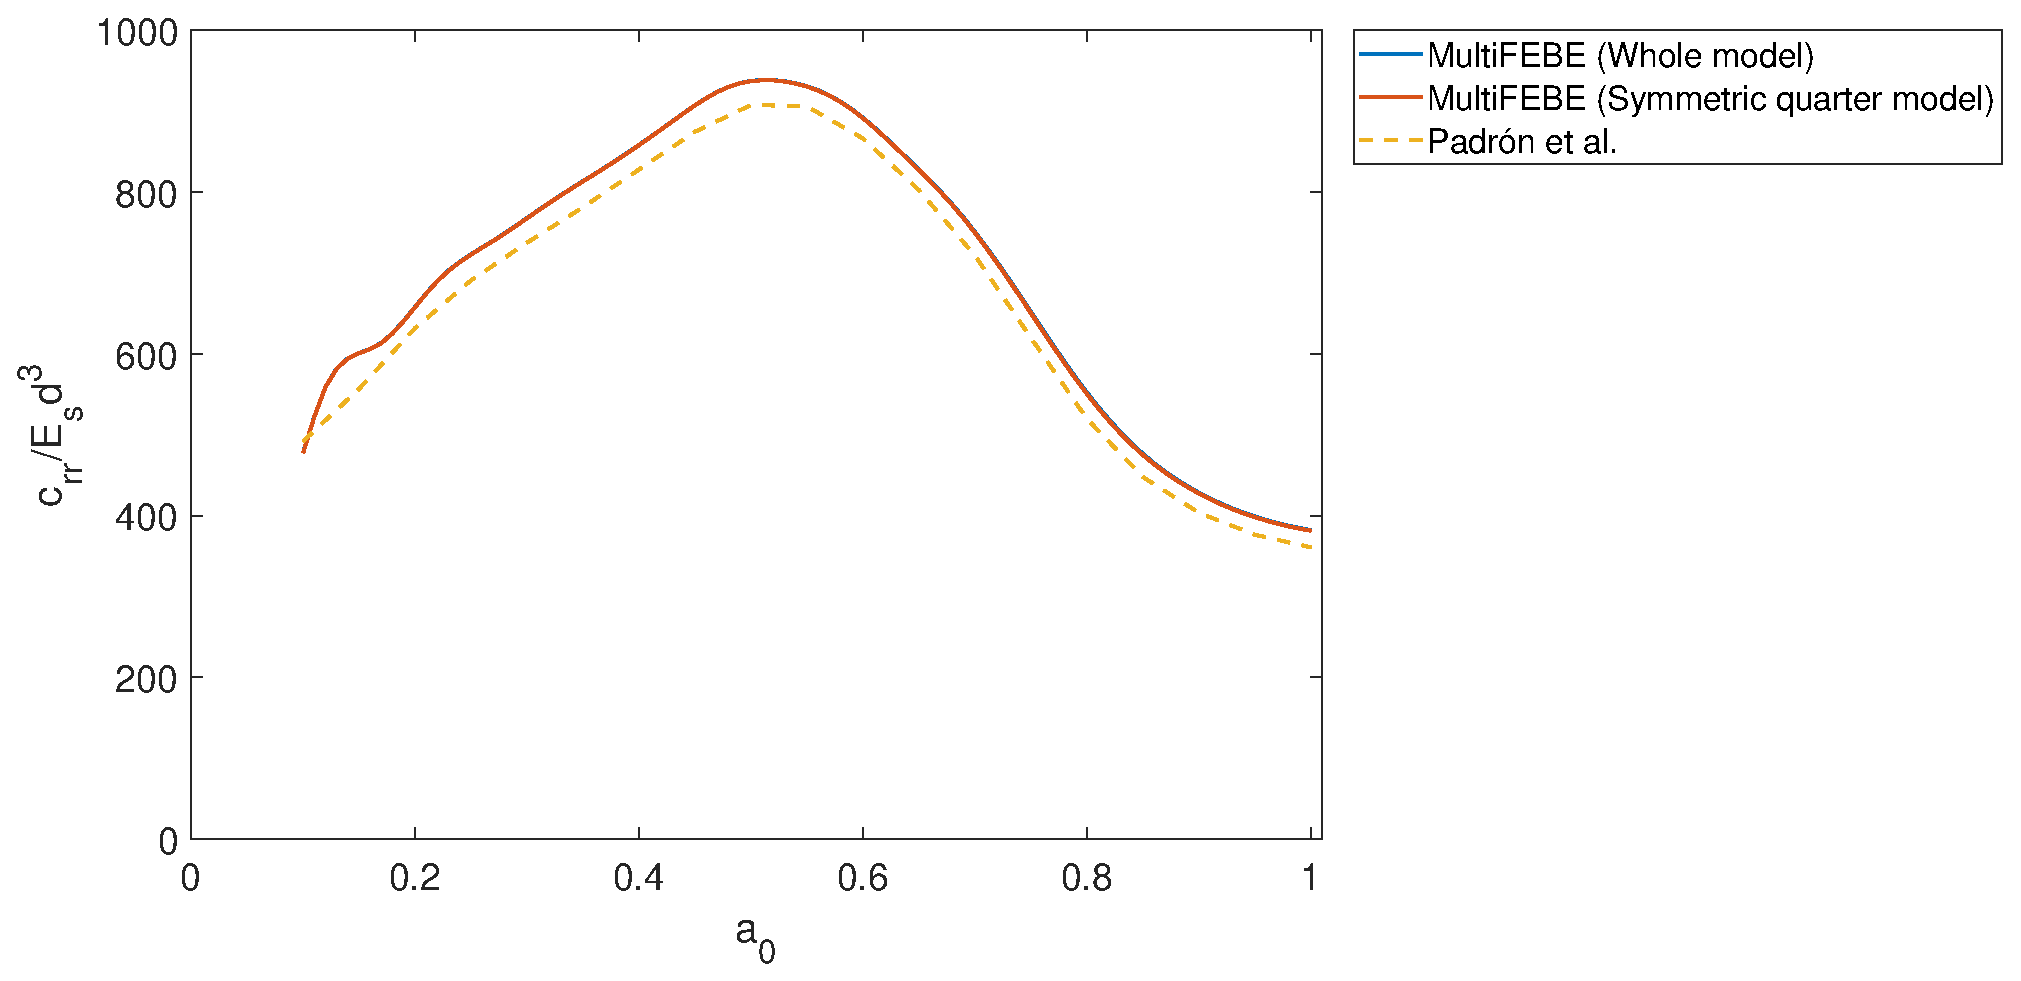
\includegraphics[scale=0.5]{crr_2x2_group.eps}
	\caption{Rocking impedance (crr).}
	\label{fig:crr_2x2_group}
\end{figure}

\FloatBarrier

\begin{thebibliography}{99}
	\bibitem{gmsh} C. Geuzaine and J.-F. Remacle, ``Gmsh: a three-dimensional finite element mesh generator with built-in pre- and post-processing facilities." \textit{International Journal for Numerical Methods in Engineering}, Volume 79, Issue 11, pages 1309--1331, (2009)
	
	\bibitem{gmshweb} C. Geuzaine and J.-F. Remacle, ``Gmsh." \url{http://gmsh.info/}
	
	\bibitem{giannakou}  A. Giannakou, N. Gerolymos and G. Gazetas, ``On the dynamics of inclined piles." \textit{Proceedings of the 10th International	Conference on Piling and Deep Foundations}, Amsterdam, The Netherlands, pages 286–-295, (2006).
	
	\bibitem{poulos} H. G. Poulos and E. H. Davis, ``Pile Foundation Analysis and Design". Wiley: New York, (1980).
	
	\bibitem{padron} L. A. Padrón, J. J. Aznárez, O. Maeso and A. Santana, ``Dynamic stiffness of deep foundations with inclined piles". \textit{Earthquake engineering and structural dynamics}, Volume 39, Issue 12, pages 1343--1367, (2010).
\end{thebibliography}

\end{document}
